Square ABCD, shown here, has side length $a$ units. Points P and Q are located on sides AD and BC, respectively, with $\text{AP}=\text{BQ}=b$ units. Triangles ACP and BDQ overlap in the square to form the shaded quadrilateral. What is the area of the shaded quadrilateral? Express your answer as a common fraction. 

\begin{figure}[H]
\centering
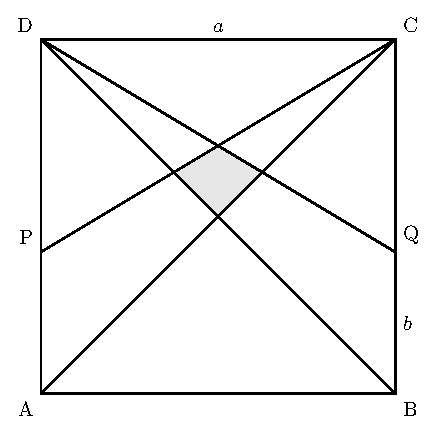
\includegraphics[height=10cm,page=1]{quadrilateral-area-shaded}
\end{figure}

